\documentclass{scrartcl}
\usepackage{amsmath}
\usepackage{float}
\usepackage[margin=1in]{geometry}
\usepackage{graphicx}
\usepackage{url}

\title{Jurassic Parkour}
\subtitle{Reinforcement Learning in an HTML5 Browser Game}
\author{Sebastian Laudenschlager, Ian Martiny}
\date{}

\begin{document}
\maketitle

\section{Introduction}

The goal of this project is to use reinforcement learning to train a computer
agent to play the Chrome T-Rex game. To that end, we use data that is
procedurally generated by running the game. The agent has a set of actions, and
the environment has a set of states, and the agent will choose an action based
on the state of the environment. To make decisions, act accordingly, and learn
from the result, we utilized the REINFORCEjs library \cite{reinforcejs}, which
implements some reinforcement learning algorithms such as Deep Q-Learning. The
platform we use to test the learning algorithm is the Javascript T-Rex game
running on a locally hosted python server using Flask. We first discuss some of
the previous related work that this project was built on, followed by a more
detailed look at the methods and algorithms we used. Subsequently, we present
some data from several experimental runs and comment on the performance of the
agent. Finally, we provide some commentary on the successes and failures of this project, as well as some ways to improve on this project.

\section{Related Work}
Our work draws from varying motivations and uses multiple resources we'd like to
acknowledge here. The two course provided sources \cite{rltutorial, rlblog} were
very helpful in learning the information necessary to use any reinforcement
learning techniques.

We examined many different tools to use for our project. Initially we attempted
to look at PyBrain~\cite{pybrain}, a \texttt{Python} library for reinforcement
learning. While promising and accomplished it we ultimately ran into issues
attempting to do our learning on a \texttt{Python} server, while the game ran on
a \texttt{JavaScript} client. Our original plan was to run the client and pass
a score to a \texttt{Python} server which then uses a reinforcement learning
library to compute new parameters. However with the nature of our game needing
to update the ``agent'' with a procedurally generated environment required a
much quicker and constant interaction between the game and the agent.

To this end we examined other projects which were based in \texttt{JavaScript}
that used reinforcement learning. One in particular that we found useful was
FlappyBirdRL~\cite{flappybirdrl}. Though it appears that this project has a self
designed reinforcement learning library tailored specifically to their project.
While interesting we were unable to adapt this to fit our needs.

Finally we examined ReinforceJS~\cite{reinforcejs}, a \texttt{JavaScript}
library for reinforcement learning. This fit our needs perfectly: a
self-contained library, meant to interact with \texttt{JavaScript} programs
directly.
\nocite{rlblogex}

\section{Methods}

    \subsection{Baselines}\label{ssec:baselines}
    Prior to testing the reinforcement learning algorithm, we established two baseline tests for
    the T-Rex game: (1) Random jumping and (2) Increasing Threshold.

    \par The random jumping baseline consists of the python server computing a random threshold
     between 0 and 1 and sending it to the Javascript client. The client then computes its own
     random threshold value between 0 and 1, and then compares the two threshold values. If the
     client's value is larger, the T-rex jumps, otherwise nothing happens. We do this for every
     run, meaning that once the T-Rex ``dies'', the game resets, and new values are computed. We
     also keep track of the score for each run, and then take the average over many runs.


    \par The increasing threshold baseline works as follows:

    \begin{itemize}
      \item If the reported score is between 1000 and 2000 (inclusive) then the new
        threshold is increased by a tenth of the distance from 1. These are
        considered low scores. A score less than 1000 is not possible. This allows
        the threshold to increase by a significant amount, without going above 1.
      \item If the reported score is between 2001 and 4000 (inclusive) then the new
        threshold is increased by a fiftieth of the distance from 1. These are still
        relatively bad scores, but realistically the best we can hope for with
        purely random jumping. For this model these scores are considered good
        enough to not change much.
      \item If the reported score is anything higher the threshold is increased by a
        hundredth of the distance from 1. Any score above 4000 is considered very
        good for this model and thus the threshold should not change very much.
    \end{itemize}

    We again keep track of the scores for many runs, and then take the average of the scores.

    \subsection{Reinforcment Learning}\label{ssec:RL}
    To actually train a computer agent to learn to play the T-Rex game, we used a reinforcement
    learning algorithm, specifically the Deep Q-Learning Algorithm from the REINFORCEjs library.
    The agent essentially learns in the following way:

    \begin{itemize}
        \item First, we initialize the agent with a set of parameters including the learning rate $\alpha$, the greedy policy $\epsilon$, the learning algorithm, experience size, etc.
        \item We then start a loop to keep playing the game. At the beginning of every run, we reset the environment states.
        \item Based on the state of the current environment, the agent chooses and executes an action.
        \item Based on the result of the action, a reward / penalty is applied.
        \item The agent then updates its policy accordingly, and if the T-Rex ``died'', the game restarts. If the agent successfully avoided an obstacle, the environment is updated to reflect the next obstacle, and the process repeats.
    \end{itemize}

    The environment states at any point in the game are described by four variables:
    \begin{itemize}
        \item The current speed of the game, i.e. how fast obstacles are moving toward the T-Rex
        \item The height (y-position) of the T-Rex
        \item The horizontal distance between the nearest obstacle and the T-Rex
        \item The height of the nearest obstacle
    \end{itemize}

    The action space for the agent is (1) Idle (do nothing), (2) Jump, and (3)
    Duck. Due to the continuous updating of the environment states, we have
    continuous state features and discrete actions, which led us to using
    REINFORCEjs's \textbf{DQNAgent}.

\section{Results}

    \subsection{Baseline}
    As reported in our Baseline report, we analyzed how ``effective'' our
    baselines were. For our baseline models we had a server-client model, where
    the server would choose the threshold for the client to jump and the client
    would report the score to the server. For our first baseline we used the
    model where the server ignored the client's score and chose a new threshold
    randomly, resulting in the following results:

    After recording the scores for 100 runs we found that the average score was
    1850.045, this corresponds to slightly better than not jumping at all.

    Our second baseline was a bit more complex, but not ``intelligent''.
    Essentially we started the client with a completely random (50\%) chance to
    jump and then slowly decreased that based on how well the client performed
    (see Section~\ref{ssec:baselines}) this baseline gave the following results:

    After recording the scores for 100 runs we found that the average score was
    1699.568, this corresponds to essentially not jumping at all. Due to the
    threshold always increasing, eventually the threshold is so large that the
    T-rex never jumps.

    \subsection{Reinforcement Learning}

    Our general methodology is discussed in Section~\ref{ssec:RL}, here we will
    discuss how our parameters were set and the results of those experiments.

    For each experiment we stored data on how the agent performed every 50
    trials, that is, in blocks of 50 trials we recorded how many successful
    jumps the agent performed, as well as the corresponding value of 
    $\epsilon$.

    Our first experiment set our learning rate $\alpha = 0.005$, and our
    greedy policy $\epsilon = 0.20$ (and slowly decreased it every action
    taken). We then chose certain actions to be rewarded and penalized as
    follows:
    \begin{align*}
        \text{idle reward} &= 3\\
        \text{success reward} &= 50\\
        \text{die penalty} & = -25
    \end{align*}
    in short, we lightly rewarded our agent for choosing to be idle (neither 
    jumping nor ducking), highly rewarded our agent for successfully jumping 
    over an obstacle and heavily penalize the agent for dying (running into an
    obstacle). These results are displayed in Figure~\ref{fig:exp1}.

    \begin{figure}[H]
        \centering
        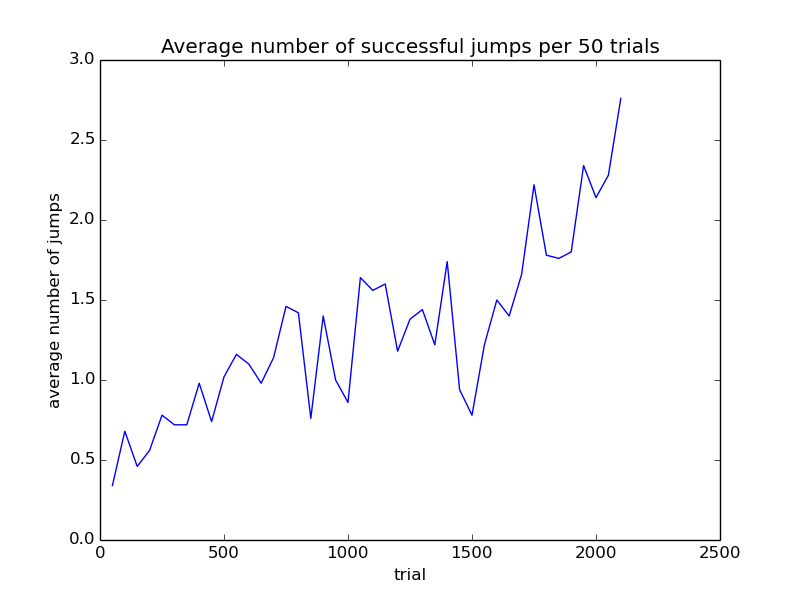
\includegraphics[width=\textwidth]{../avgJumps1}    
        \caption{Average number of successful jumps with $\alpha = 0.005$, no
        jump penalty, idle reward = $3$, success reward = $50$, and dying
        penalty = $-25$}
        \label{fig:exp1}
    \end{figure}

    Our second experiment changed essentially nothing except that we imposed a
    jumping penalty to our agent, of $-10$, hoping to curb the agent's
    enthusiasm to continuously jump. These results are displayed in Figure~
    \ref{fig:exp2}.

    \begin{figure}[H]
        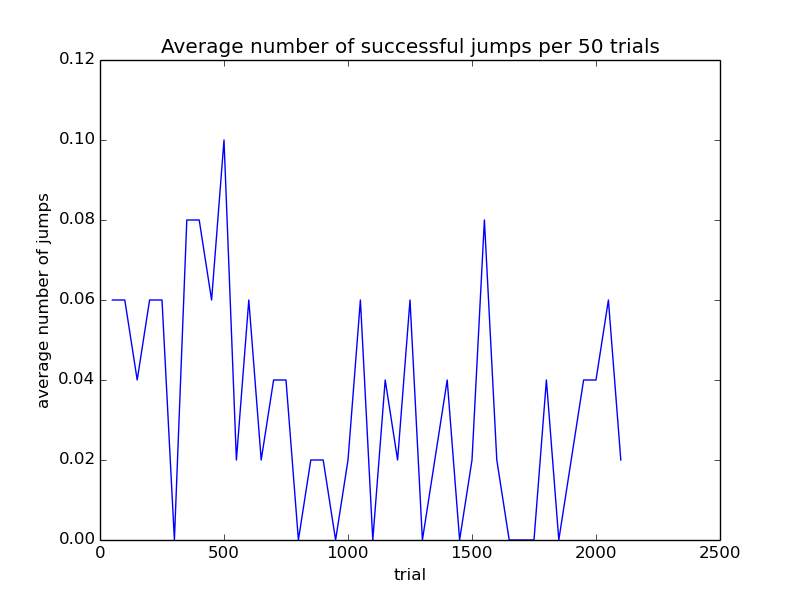
\includegraphics[width=\textwidth]{../avgJumps2}    
        \caption{Average number of successful jumps with $\alpha = 0.005$,
        jump penalty = $-10$, idle reward = $3$, success reward = $50$, and
        dying penalty = $-25$}
        \label{fig:exp2}
    \end{figure}

    Our final two experiments were with randomized values for our features, in
    an attempt to examine the effect of various changes to parameters.

    Experiment three had the following settings:
    \begin{align*}
        \alpha &= 0.8682662725534351\\
        \text{jump penalty} &= -7\\
        \text{idle reward} &= 4\\
        \text{success reward} &= 11\\
        \text{die penalty} & = -16
    \end{align*}
    The results of this experiment are displayed in Figure~\ref{fig:exp3}.

    \begin{figure}[H]
        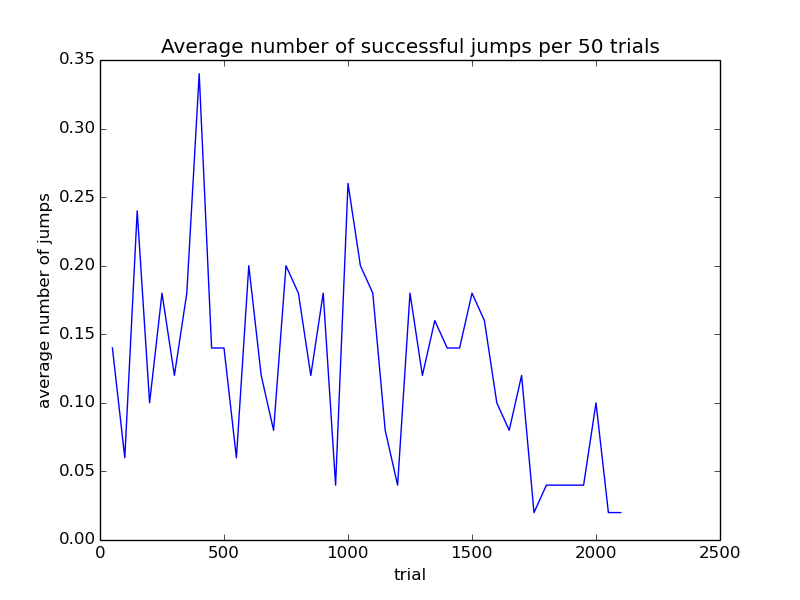
\includegraphics[width=\textwidth]{../avgJumps3}    
        \caption{Average number of successful jumps with $\alpha =
        0.8682662725534351$, jump penalty = $-7$, idle reward = $4$, success
        reward = $11$, and dying penalty = $-16$}
        \label{fig:exp3}
    \end{figure}

    Experiment four had the following settings:
    \begin{align*}
        \alpha &= 0.6564771414639463\\
        \text{jump penalty} &= -4\\
        \text{idle reward} &= 4\\
        \text{success reward} &= 34\\
        \text{die penalty} & = -18
    \end{align*}
    The results of this experiment are displayed in Figure~\ref{fig:exp4}.

    \begin{figure}[H]
        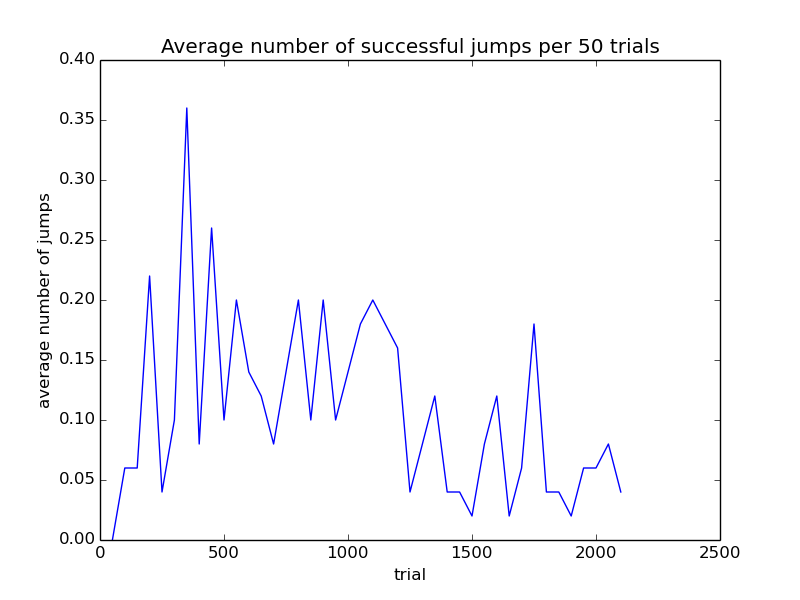
\includegraphics[width=\textwidth]{../avgJumps4}    
        \caption{Average number of successful jumps with $\alpha =
        0.6564771414639463$, jump penalty = $-4$, idle reward = $4$, success
        reward = $34$, and dying penalty = $-18$}
        \label{fig:exp4}
    \end{figure}

    \subsection{Discussion}
    As can be seen from our graphs, none of our experiments were able to
    correctly ``solve'' the T-Rex game. While our first experiment was able to
    average around 3 successful jumps per trial future experiments were more
    chaotic and did not perform as well.


\section{Conclusion}

\bibliographystyle{unsrt}
\bibliography{sources}

\end{document}
